% This must be in the first 5 lines to tell arXiv to use pdfLaTeX, which is strongly recommended.
\pdfoutput=1
% In particular, the hyperref package requires pdfLaTeX in order to break URLs across lines.

\documentclass[11pt]{article}

% Remove the "review" option to generate the final version.

\usepackage{acl}
\usepackage{amsmath}
\usepackage{graphicx}
\usepackage{subcaption}
\usepackage{booktabs}
\usepackage{url}
% Standard package includes
\usepackage{times}
\usepackage{latexsym}
\usepackage{xcolor}


% For proper rendering and hyphenation of words containing Latin characters (including in bib files)
\usepackage[T1]{fontenc}
% For Vietnamese characters
% \usepackage[T5]{fontenc}
% See https://www.latex-project.org/help/documentation/encguide.pdf for other character sets

% This assumes your files are encoded as UTF8
\usepackage[utf8]{inputenc}

% This is not strictly necessary, and may be commented out,
% but it will improve the layout of the manuscript,
% and will typically save some space.
\usepackage{microtype}

% If the title and author information does not fit in the area allocated, uncomment the following
%
%\setlength\titlebox{<dim>}
%
% and set <dim> to something 5cm or larger.







\title{Project Report: On-device Speech Translation}

% Author information can be set in various styles:
% For several authors from the same institution:
% \author{Author 1 \and ... \and Author n \\
%         Address line \\ ... \\ Address line}
% if the names do not fit well on one line use
%         Author 1 \\ {\bf Author 2} \\ ... \\ {\bf Author n} \\
% For authors from different institutions:
% \author{Author 1 \\ Address line \\  ... \\ Address line
%         \And  ... \And
%         Author n \\ Address line \\ ... \\ Address line}
% To start a seperate ``row'' of authors use \AND, as in
% \author{Author 1 \\ Address line \\  ... \\ Address line
%         \AND
%         Author 2 \\ Address line \\ ... \\ Address line \And
%         Author 3 \\ Address line \\ ... \\ Address line}

\author{
  Team Jobless\\
  Jiyang Tang (jiyangta), Ran Ju (ranj), Tinglong Zhu (tinglonz), Xinyu Lu (xinyulu2)\\
}

\begin{document}
\maketitle

\begin{abstract}

This project aims to develop an efficient on-device speech translation system, addressing the challenge of language barriers in a globalized society. Traditional translation methods can be cumbersome, particularly in areas with limited internet access. Our solution emphasizes on-device translation to enhance privacy, reduce latency. The crucial part of our approach is the implementation of model compression techniques, specifically quantization and pruning based on ESPNet, which are crucial for the deployment of efficient real-time systems on devices with limited computational resources. We further refine our system's efficiency by applying the Open Neural Network Exchange (ONNX) optimizations. Our methods resulted in a 62\% reduction in latency and a 73\% reduction in model size, with a trade-off of a 25\% decrease in BLEU score, indicating a significant improvement in efficiency with a modest degradation in translation accuracy. These techniques do not require re-training the model and can be implemented easily using PyTorch and ONNX libraries.
\end{abstract}




\section{Introduction}
Language barriers are a common obstacle faced by travelers around the world. In an increasingly globalized society, the ability to communicate with people from diverse linguistic backgrounds is crucial for social interaction, tourism, business, and emergency situations. Traditional phrasebooks and online translation services can be cumbersome, especially in areas with limited internet connectivity. 

On-device speech translation aims to bridge this gap. On-device machine learning has gained popularity due to its potential to enhance privacy and reduce latency. Deploying machine learning models on user devices reduces the reliance on centralized servers, improving the user experience and alleviating concerns about data security and privacy. Personal conversations and sensitive information are not transmitted to external servers, reducing the risk of data breaches or unauthorized access. What's more, nowadays edge device has sufficient power to run models offline, and deploying the models on the devices directly is helpful in reducing latency.

In this project, our objective is to build and deploy an end-to-end speech translation system to a laptop based on ESPnet. We try to tackle the challenge of designing and developing targeted methods of pruning and quantization tailored to ESPnet-based model. This approach is essential to ensure the deployment of the model on laptop devices with both acceptable inference latency and performance. We also run experiments to see how the model efficiency will affect the power consumption.


\section{Related Works}\label{sec:related_work}

For speech translations (ST), there are mainly two approaches: cascaded ST system and end-to-end (E2E) ST systems (E2E-ST). For the cascaded ST, the idea is to split the speech translation task into smaller and feasible sub-tasks: speech translation and machine translation \cite{xu2023recent}. While E2E-ST aims to solve the speech translation problem with an E2E model. Both approaches have their problems. Cascaded systems have the issue of error accumulation while the E2E ST model is difficult to learn due to the cross-lingual and cross-modal mapping in a single model \cite{xu2023recent}.


% For cascaded systems, the latest systems are composed of Transformer/Transformer Variants (including Speech-Transformer, Conformer, self-supervised learned Transformer, like Wave2Vec, HuBERT, etc.) based ASR, and Transformer-based MT (since Transformer architecture outperforms all the other model architectures in sequence generation task) \cite{xu2023recent}. 

For E2E-ST, researchers usually use a multitask framework to train the model, since the cross-lingual and cross-modal mapping make the training process much more challenging compared to training the sub-modules independently \cite{xu2023recent}. There are several training strategies: decoupled decoder, decoupled encoder, and two-stream encoder. The decoupled decoder strategy reduces the modeling burden by adding a speech recognition (ASR) decoder in addition to the machine translation (MT) decoder. For the decoupled encoder strategy, it adds an additional semantic encoder to the original pipeline. Other than directly encoding speech into semantic features, it eases the encoder’s burden by first encoding speech into acoustic features and then encoding it into semantic features. Two-stream encoder approach adds a shared encoder, which takes either output from a speech encoder or machine translation text encoder, and its outputs will be used to generate translated text. This aims to map the speech encoder’s feature space and the text encoder’s feature space into the same one, which makes it easier to train the whole E2E-ST system. 


% The BLEU score for the cascaded systems and E2E-ST are shown in Table \ref{Table: acc}.
% \begin{table}[h]
% \begin{tabular}{lll}
% \hline
% Model    & Fisher (test) & CallHome (evltest) \\ \hline
% E2E-ST   & 50.86         & 19.36              \\
% Cascaded & 42.16         & 19.82              \\ \hline
% \end{tabular}
% \caption{BLEU scores of the cascaded and end-to-end translation systems.}
% \label{Table: acc}
% \end{table}

Recently, a lot of work has been done on ASR/MT compression (most of them are quantization and pruning metrics, such as ~\cite{see2016compression}), but little work has been done on ST model compression. We believe these techniques also apply to the ST task. 




\section{Task Definition and Problem Setup}\label{sec:definition}

\paragraph{Model}
In this project, our investigations focus on E2E-ST. We chose the decoupled decoder scheme mentioned above. In this scheme, the ASR decoder is not required during inference which removes some computation burden.
Specifically, we have an speech encoder that extract high-level vector representations from the input speech features (FBank). Then the MT decoder predicts the next token based on the previous token sequence while attending to the encoder output. 

Due to the heavy computation requirement for re-training the models, we utilize a pre-trained model from HuggingFace. The details about this model will be specified in later sections.


\paragraph{Dataset}
For the dataset, we use MuST-C~\cite{di2019must} for benchmarking experiments. MuST-C is a corpus designed for speech translation, primarily focusing on translating TED talks from English into several other languages. It is a multilingual dataset that provides sentence-level parings of speech and text. We utilize the English-to-Dutch language pairs from its test set to evaluate latency and translation accuracy. 


\paragraph{Evaluation metric}
In order to measure the accuracy-performance trade-offs, it is crucial to employ robust evaluation metrics that effectively encapsulate the quality and efficiency of generated outputs. For our project, we selected BLEU (Bilingual Evaluation Understudy) and latency as our primary metrics.
\textbf{BLEU} is a widely accepted metric in the translation community, known for measuring the correspondence of n-grams between machine-generated translations and their reference counterparts. A higher BLEU score indicates better performance.

However, while \textbf{BLEU score} effectively assesses translation accuracy, it does not evaluate the operational efficiency of the translation system. Therefore, we use \textbf{latency} as a significant metric. Latency measures the time taken for the system to produce the translation with the provided input. A lower \textbf{latency} indicates a more efficient system that offers faster translations.
We also measure Floating-Point Operations per Second (FLOPS) for some experiments where we can get an accurate measurement using GPU and \texttt{deepspeed}\footnote{\url{https://github.com/microsoft/DeepSpeed}} library. This metric measures how fast calculations are performed and can reflect whether the model is utilizing the underlying hardware efficiently.


\paragraph{Hardware} The hardware we are targeting at is a Dell G15 5511 laptop. Its specifications are shown below:
\begin{enumerate}
    \item CPU
    \begin{enumerate}
        \item 11th Gen Intel i7-11800H, 2.30GHz
        \item Speed 3.35 GHz
        \item 8 cores, 16 logical processors
        \item L1 cache: 640 KB
        \item L2 cache: 10.0 MB
        \item L3 cache: 24.0 MB
    \end{enumerate}
    \item GPU
    \begin{enumerate}
        \item NVIDIA GeForce RTX 3060 Laptop GPU/PCIe/SSE2  
        \item Driver: NVIDIA 470.223.02
        \item CUDA 12.3
    \end{enumerate}
    \item Memory: 32GB, dual-channel DDR4
    \item OS: Linux 6.2.0-37-generic x86 64-bit, Ubuntu 22.04.3 LTS
    \item Python environment:
    \begin{enumerate}
        \item Python==3.10
        \item PyTorch==2.0.1
        \item ESPnet==202308
    \end{enumerate}
\end{enumerate}




\section{Methods}

Deploying deep learning models on devices for real-time applications poses a significant challenge due to their computation and storage overhead. To address this challenge, we explore two techniques: quantization and pruning.
Quantization reduces the precision of the model’s weights in exchange for faster computation and smaller memory footprint. Meanwhile, pruning eliminates parts of the network to reduce the total computation operations. Both techniques aim to reduce the model’s size and computational demands but potentially compromise the translation accuracy.
We are curious about how much quantization and pruning we can apply to create a lightweight and efficient speech translation system.

Another aspect of our research is the choice of representation and interchange formats for neural network models.
There are many software that optimizes the inference process of ML models.
Typical optimization techniques include but are not limited to computation graph optimization and multi-threading.
In addition, these inference engines can decouple our model from the dependency on ESPnet, which makes deployment on smaller devices much more convenient.
Our research objective is to export our model to the ONNX format and use ONNX runtime to perform inference. We are interested to see its impact on latency, translation accuracy, and model size.

Furthermore, speech recognition relies on the efficient representation and processing of audio signals. Speech encoders usually use convolution layers to consolidate input features into subsampled high-level representations. This reduces the computation needed since the sequence length is reduced. In this part, we seek to find a method that can increase the subsampling rate without significantly compromising the performance.

\subsection{Baseline}

To save time, we utilize a pre-trained model\footnote{\url{https://huggingface.co/espnet/brianyan918_mustc-v2_en-de_st_conformer_asrinit_v2_raw_en_de_bpe_tc4000_sp}} from Hugging Face Hub for our experiments.
As described in Section~\ref{sec:related_work} and Section~\ref{sec:definition},
this E2E-ST system is an encoder-decoder model with multitask training objectives~\cite{inaguma2020espnet}.
The encoder is a Conformer~\cite{conformer} with $12$ layers, each having $4$ attention heads and $2048$ hidden units.
The MT decoder is a Transformer~\cite{transformer} with $6$ layers, each containing $4$ attention heads and $2048$ hidden units.
Both the encoder and the decoder use a dropout rate of $0.1$ for positional encoding and attention.
The beam size is set to $10$ during inference.

\subsection{Reduce Input Size}
We propose two methods to decrease input size.
For the first method, we change the hop length of the sliding windowing function when calculating FBank features. The larger the hop length is, the more windows are spread out, and thus the smaller the input size is. However, the sampling rate within each window remains the same, therefore this technique is unlikely to cause huge information loss.

Another way to vary the input size is to reduce the sample rate from 16k to 8k using the ffmpeg toolkit. This can be combined with the first method to further shrink the input size. We aim to explore if subsampling the original wav can lower the input size without significantly harming the performance.


\subsection{Quantization}
We believe Post-Training Quantization is most suitable for this project, since Quantization-Aware Training (QAT) is not realistic because we do not have sufficient resources to train this model. 
PTQ is shown to be quite effective for many speech tasks, and we believe with proper implementation and tuning, we can achieve a big reduction of model size and inference latency.
We plan to quantize the model using 8-bit integer instead of 16-bit float, because the PyTorch CPU backend does not provide native support for such data types, and our experiments in later sections show that these types actually increase the latency.

In addition, our investigations are focused on dynamic quantization instead of static quantization.
Static quantization requires calibration which is difficult to implement due to ESPnet's complexity. During beam search, we need to quantize and dequantize the input and output of the MT decoder for each step. This requires a substantial change to ESPnet's internal code, and we simply didn't have enough time. 


\subsection{Pruning}
For our project, we apply unstructured L1 magnitude pruning to our model. We experiment with global pruning and component-wise pruning with different sparsity to find the best pruning strategy for this task. Our goal is to reduces the inference latency as much as possible without damaging the translation quality.



\subsection{ONNX Runtime}
As explained above, we use ONNX to export our models and perform inference using ONNX runtime.
We use \texttt{espnet\_onnx}\footnote{\url{(https://github.com/espnet/espnet_onnx)}} library to assist us exporting the encoder and the decoder separately. The original ESPnet codebase has a lot of operations like lambda and argument unpacking, which \texttt{torch.onnx.export} fails to deal with automatically. In addition, \texttt{espnet\_onnx} can help us specify the dynamic input dimensions automatically.

\subsection{Combining All Techniques}

We are interested to see whether combining the techniques mentioned above can further increase the efficiency of our models.
We aim to investigate how these techniques affect each other in terms of inference latency and model sizes.
For example, combining pruning with ONNX runtime can potentially reduce the number of calculations because ONNX can fuse pruned modules together can increase sparsity even more.

\subsection{Measuring Energy Use}
We measure the energy use of our model on the two platforms which are laptop CPU and laptop GPU. For laptop CPU, we use CodeCarbon combined with Intel RAPL (Running Average Power Limit) Interface to measure energy consumption. It provides both a high-level estimation of energy use and a more detailed measurement of CPU. This approach can account for the total energy consumed by the system and the specific energy use of model inference. For laptop GPU, we use CodeCarbon combined with PyNVML. In this way, it can directly query the GPU for its power state, which is crucial for an accurate assessment of energy consumption.

We use a test dataset of 100 utterances to benchmark our model. For each experiment, we run the inference on the test dataset four times to get a stable estimate. We repeated the experiment five times to report the mean and standard deviation of the energy consumption per utterance. We set our batch size to 1, since out model is an auto-regressive model which can accept input with different lengths. Thus, it is hard for us to implement efficient batch inference (ESPnet does not support batch inference well, either). We start our power measurement when the model starts inferencing the first sample, and stop measuring when the model finishes inferencing all the samples. Since there is very little overhead between the inference of two samples, we decided to ignore this part's energy consumption. We decided not to perform measurements at the wall (since we use PC platform).

\section{Results and Discussion}

\begin{figure*}[h]
    \centering
    \begin{subfigure}{0.32\textwidth}
        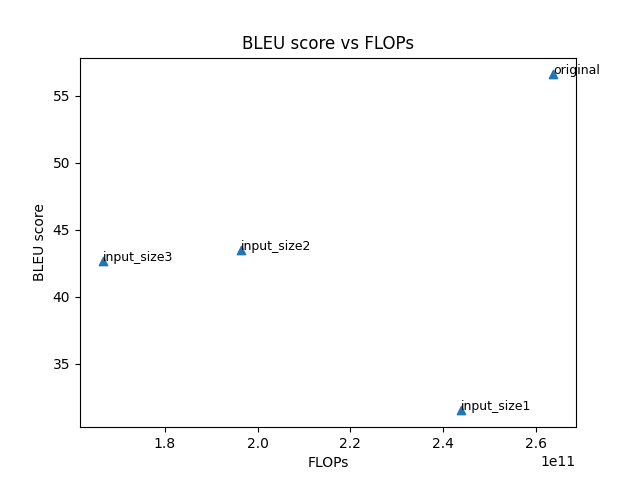
\includegraphics[width=\textwidth]{images/input_size/BLEU_vs_FLOP.png}
        \caption{FLOPs vs. BLEU}
    \end{subfigure}
    %\hfill % adds horizontal space between the images
    \begin{subfigure}{0.32\textwidth}
        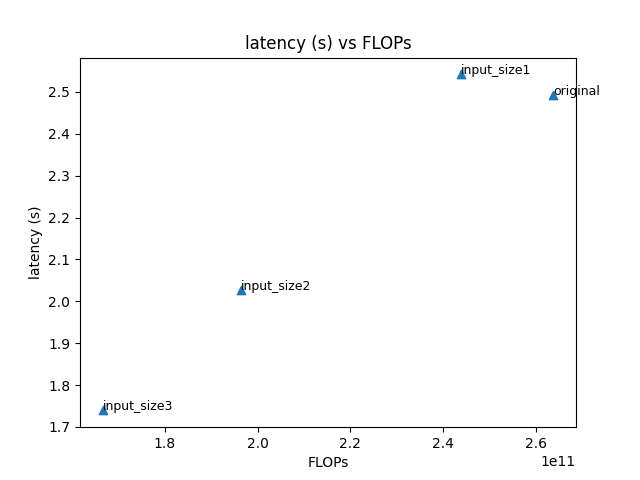
\includegraphics[width=\textwidth]{images/input_size/latency_vs_FLOP.png}
        \caption{FLOPs vs. Latency}
    \end{subfigure}
    %\hfill % adds horizontal space between the images
    \begin{subfigure}{0.32\textwidth}
        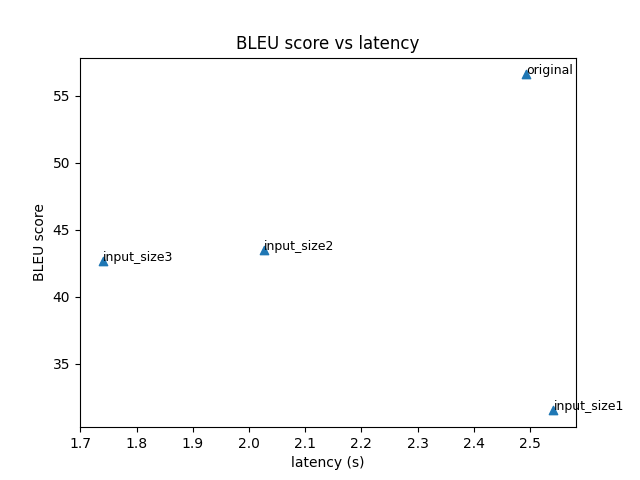
\includegraphics[width=\textwidth]{images/input_size/BLEU_vs_latency.png}
        \caption{Latency vs. BLEU }
    \end{subfigure}
    \caption{\label{fig:input_size}Comparative Plots For Different Input Size (Method 1)}
\end{figure*}


\begin{figure*}[h]
    \centering
    \begin{subfigure}{0.32\textwidth}
        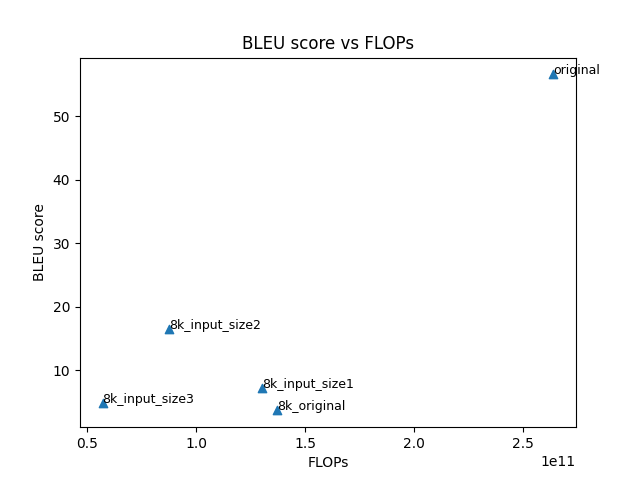
\includegraphics[width=\textwidth]{images/input_size_method2/BLEU_vs_FLOP.png}
        \caption{FLOPs vs. BLEU}
    \end{subfigure}
    %\hfill % adds horizontal space between the images
    \begin{subfigure}{0.32\textwidth}
        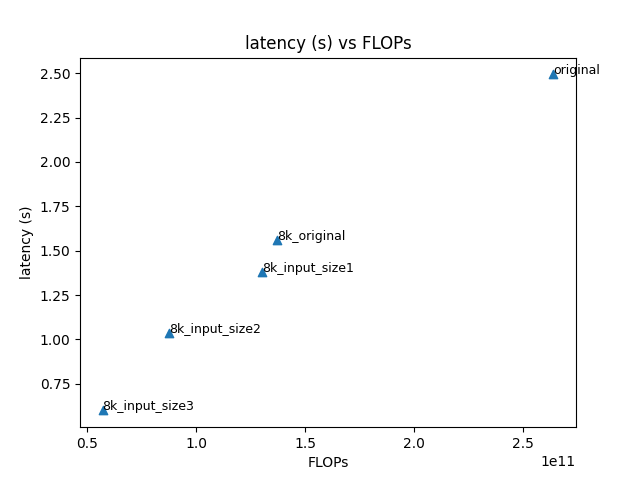
\includegraphics[width=\textwidth]{images/input_size_method2/latency_vs_FLOP.png}
        \caption{FLOPs vs. Latency}
    \end{subfigure}
    %\hfill % adds horizontal space between the images
    \begin{subfigure}{0.32\textwidth}
        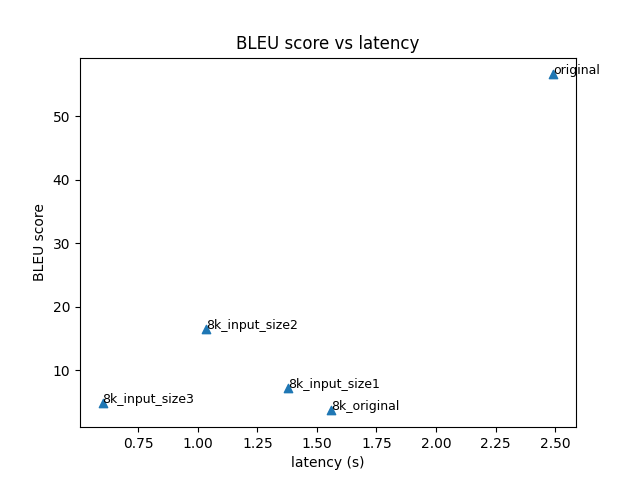
\includegraphics[width=\textwidth]{images/input_size_method2/BLEU_vs_latency.png}
        \caption{Latency vs. BLEU }
    \end{subfigure}
    \caption{\label{fig:input_size_method2}Comparative Plots For Different Input Size (Method 2)}
\end{figure*}

In this section, we present our experimental results and discuss their implications.
All experiments were conducted using ESPnet~\cite{espnet}.

\subsection{Varying Input Size}

The hop length and sampling rate for each experiment are shown in Table \ref{tab:vary_input_size}.
The experiment results for our first method (increase hop length only) are shown in Figure \ref{fig:input_size}. From the BLEU score vs FLOPs plot we observe that as we decrease the input size, the FLOPs decrease as expected. As the FLOPs decrease, we don't see a clear trend of increasing or decreasing BLEU scores. We think the reason is that we didn't re-train the model after changing the hop length. Since the model is trained using a hop length of 160 (16KHz wav), inference with different hop lengths will affect and bring a lot of uncertainty to the BLEU score performance. 

The BLEU score vs latency graph looks similar to the BLEU score vs FLOPs one. The latency decreases as we decrease the input size. The BLEU score also drops as we change the input size because of the loss of information brought by increasing the hop length and the mismatch between the training and inference features (led by different hop length).

For the relationship between FLOPs and latency, we find that latency increases as the FLOPs increases as expected.  

We observe an interesting phenomenon for input\_size1: its latency is higher than the original method, but its BLEU score is much lower than that of the original and input\_size2 and input\_size3. We hypothesize that this is because of the inconsistency between the training and inference features. The model produces bad quality outputs without stopping tokens until it reaches the maximum output length, resulting in higher latency and very low BLEU score.

For the second way of varying input size (first subsample the original wav and then increase the hop length), the experiment results are shown in Figure~\ref{fig:input_size_method2}. By examining the graph depicting the relationship between BLEU score and FLOPs, it is apparent that reducing the input size leads to the expected decrease in FLOPs. However, as FLOPs decrease, there isn't a discernible pattern of either an increase or a decrease in the BLEU score. The graph illustrating the relationship between BLEU score and latency closely resembles the one comparing BLEU score to FLOPs. As the input size decreases, latency also decreases. The BLEU score tends to decrease when adjusting the input size due to disparities between the training and inference input sizes, although there isn't a clear, consistent trend observed. When examining the connection between FLOPs and latency, we generally observe that as FLOPs increase, latency also tends to increase.


In the analysis of the experiment results of the two methods, we observe that in terms of the BLEU score, if we decrease the sample rate by half, the BLEU score drops dramatically, except input\_size2, the BLEU scores for all other models drop to less than 10. We think the reason is that the dropped samples would cause the inconsistency between the training and inference input features. For example, The model was trained with normal speech rate data, and he may not recognize accelerated speech (subsampling the raw wav and increasing the hop length is similar to accelerate the speech) very well. Failing to correctly recognize the speech will negatively affect the translation quality. In terms of latency, we find that if we decrease the sample rate first, the latency will decrease significantly. It is as expected because there is less computation. In all, we think decreasing the sample rate is not a good strategy for decreasing the input size since the BLEU score drops too much. In comparison, changing hop length directly has a better trade-off between performance and latency. 

\begin{table}
\centering
\small
\begin{tabular}{cc}
\toprule  
\textbf{Model} & \textbf{Hop length}\\
\midrule 
original & 160\\
input\_size1 & 200\\
input\_size2 & 250\\
input\_size3 & 300\\
\bottomrule
\end{tabular}
\caption{Experiments of Varying Input Size}
\label{tab:vary_input_size}
\end{table}


\subsection{Quantization}

\begin{table}[ht]
\centering
\resizebox{0.95\linewidth}{!}{
\begin{tabular}{|c|c|c|c|c|c|c|}
\hline
\textbf{Configuration} & \textbf{Q} & \textbf{dtype} & \textbf{Size (MB)} & \textbf{Params} & \textbf{BLEU} & \textbf{Latency(s)} \\ \hline
Original               & -          & float32        & 220                & 57,592,032      & 56.6          & 1.41                \\ \hline
input\_size1           & -          & float32        & 220                & 57,592,032      & 31.5          & 1.24                \\ \hline
input\_size2           & -          & float32        & 220                & 57,592,032      & 43.5          & 1.10                \\ \hline
input\_size3           & -          & float32        & 220                & 57,592,032      & 42.7          & 0.97                \\ \hline
Original               & D          & qint8          & 70                 & 57,592,032      & 35.8          & 1.20                \\ \hline
input\_size1           & D          & qint8          & 70                 & 57,592,032      & 35.8          & 1.06                \\ \hline
input\_size2           & D          & qint8          & 70                 & 57,592,032      & 43.5          & 0.96                \\ \hline
input\_size3           & D          & qint8          & 70                 & 57,592,032      & 37.2          & 0.92                \\ \hline
Original               & D          & float16        & 220                & 57,592,032      & 56.6          & 2.05                \\ \hline
input\_size1           & D          & float16        & 220                & 57,592,032      & 31.5          & 1.76                \\ \hline
input\_size2           & D          & float16        & 220                & 57,592,032      & 43.5          & 1.53                \\ \hline
input\_size3           & D          & float16        & 220                & 57,592,032      & 42.6          & 1.40                \\ \hline
\end{tabular}
}
\caption{Quantization under different settings.}
\label{table:model_benchmarks}
\end{table}


We performed three sets of experiments:
\begin{itemize}
    \item  Baselines without quantization
    \item Dynamic PTQ with 8-bit (integer) precision
    \item Dynamic PTQ with 16-bit (float) precision
\end{itemize}

Figure \ref{fig:prun_module_all} shows our results with each set of experiments marked with different colors:

There are several interesting conclusions (with and without PTQ, and using different precisions) we can draw from this plot: decreasing the input size reduces the inference latency regardless of whether quantization is enabled.

Dynamic PTQ using 8-bit integer significantly reduces the inference latency.
However, it also reduces the BLEU score, especially when the input size isn't reduced (comparing \textit{original} in blue and
green).
Moreover, the difference in latency is less significant when the input size becomes smaller (for example,
comparing \textit{original} and \textit{input\_size3} in blue and green).
Strangely, \textit{input\_size2} with 8-bit integer PTQ achieves higher BLEU score than other reduced input size experiments
even without PTQ.
We believe somehow this configuration introduces the least precision loss, showing that calibration is very important for PTQ.
Overall, this level of decrease in BLEU score is acceptable for our project.
But we will try to improve this using static PTQ in the future.

Another interesting finding is that dynamic PTQ using 16-bit float drastically increase the inference latency.
Meanwhile, the BLEU scores stay the same as the baselines.
The reason is that X86 PyTorch backend doesn't natively support FP16, therefore needs to emulate 16-bit precision using FP32.
Also, speech translation models have more diverse layers and that requires more value conversions, causing the latency to increase without the benefit of reduced model size.
Since our target platform is X86 CPUs, we will not use this type of quantization in the final product.




\subsection{Prunning}
\subsubsection{Global Prunning}
For this experiment (results shown in Table \ref{tab: whole_model_tab}), we did not iteratively prune the entire model with 33\% of the remaining parameters each time. Since we found that the performance degradation is huge when the sparsity is becoming larger and larger, and iteratively pruning the model would cause the sparsity of the model to rapidly approach 0.9. The BLEU score is less than 10 when the sparsity is large or equal to 0.5. And when the sparsity is large or equal to 0.9, the BLEU score becomes zero, meaning that the output of the model makes no sense. Thus conduct the experiment on the sparsity.

\begin{table}[h!]
\centering
\resizebox{0.95\linewidth}{!}{
\begin{tabular}{ccccc}
\cline{2-5}
\hline
Experiment ID& Sparsity & BLEU     & Latency (s) & Disk Size (MB) \\ \hline
0 & 0        & 56.59119 & 1.406278    & 220            \\ 
1 & 0.1      & 56.59119 & 1.392705    & 842            \\
2 & 0.2      & 56.59119 & 1.324602    & 753            \\
3 & 0.33     & 29.50234 & 1.43281     & 639            \\
4 & 0.4      & 26.2691  & 0.81771     & 577            \\
5 & 0.5      & 3.379674 & 6.36895     & 490            \\
6 & 0.6      & 2.747578 & 6.283118    & 402            \\
7 & 0.7      & 1.349908 & 6.568361    & 314            \\
8 & 0.8      & 0.679364 & 6.227498    & 226            \\
9 & 0.9      & 0        & 6.228       & 138            \\ \hline
\end{tabular}
}
\caption{Results of Global L1 Unstructured Pruning}
\label{tab: whole_model_tab}
\end{table}


\begin{figure*}[h!]
    \centering
    \begin{subfigure}{0.45\textwidth}
        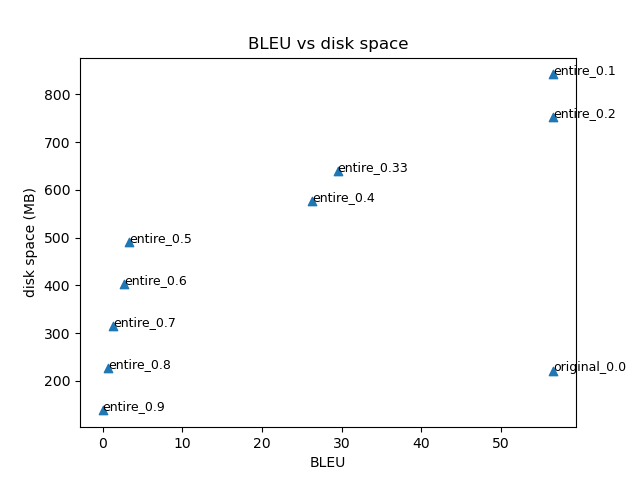
\includegraphics[width=\textwidth]{images/prun_whole_model/BLEU_vs_disk_space.png}
        \caption{BLEU vs. Disk Space (MB)}
    \end{subfigure}
    %\hfill % adds horizontal space between the images
    \begin{subfigure}{0.45\textwidth}
        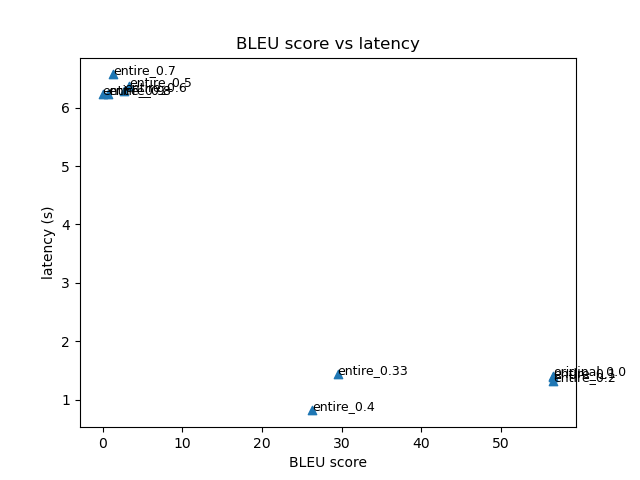
\includegraphics[width=\textwidth]{images/prun_whole_model/BLEU_vs_latency.png}
        \caption{BLEU vs. Latency (s)}
    \end{subfigure}
    %\hfill % adds horizontal space between the images

    \centering
    \begin{subfigure}{0.5\textwidth}
        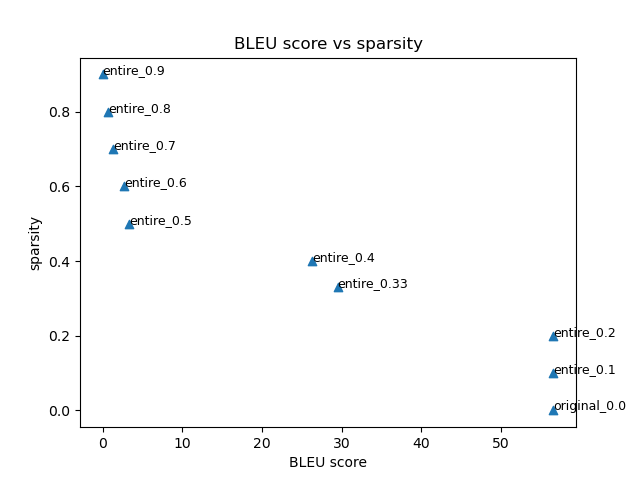
\includegraphics[width=\textwidth]{images/prun_whole_model/BLEU_vs_sparsity.png}
        \caption{BLEU vs. Sparsity}
    \end{subfigure}
    \caption{\label{fig:whole_model_prun_3fig}BLEU scores, latency and disk space of globally pruned models with different sparsity settings}
\end{figure*}
From the experiment results (Table. \ref{tab: whole_model_tab}) and the 3 plots (Figure. \ref{fig:whole_model_prun_3fig}), we can get to the following conclusions:
\begin{enumerate}
    \item Only when the model’s sparsity is larger than 0.8, the model’s disk space usage will be smaller than the original model, while when the sparsity is small (such as 0.1, 0.2) the model’s disk space consumption will far larger than that of the original model. We consider it to be the same reason as mentioned in Part I.
    \item When the model’s sparsity is getting larger and larger, the model’s latency in fact increases. Since the model’s performance degrades as the sparsity gets larger, the auto-regressive model’s stop predictor will become worse and worse, thus when the model’s sparsity is getting larger, the model is more likely not to stop at the right point and will continuously generate output until reaches the maximum length. Thus, the latency increases as the sparsity gets larger.
    \item For the BLEU score vs. sparsity. We could see that the BLEU score of the model whose sparsity is less or equal to 0.2 is really close to that of the original model. We think that it is the true pruning, which prunes out some of the unnecessary or redundant parameters (having small magnitude). But when the sparsity of the model gets larger and larger, more and more the important parameters are pruned out, which causes huge performance degradation. If we retrain the model while pruning, we might be able to achieve higher sparsity while keeping an acceptable performance loss.
\end{enumerate}

\subsubsection{Sensitive Analysis of Different Components of the Model}
Here we conduct experiments on unstructured pruning of different components:
\begin{enumerate}
    \item Encoder's or decoder's:
    \begin{enumerate}
        \item feed forward layers (ff)
        \item point/depth-wise convolution layer + batch normalization (conv)
        \item self-attention, including the linear transformations (self\_attn) 
        \item layer normalizations (norm)
    \end{enumerate}
    \item Encoder’s subsampling module (modules that reduces sequence length)
    \item Decoder’s cross attention module
    \item Decoder’s embedding module.

\end{enumerate}

For the modules listed above, we conducted experiments pruning each module (L1 unstructured pruning) at 0.33, 0.5, 0.7, 0.9 sparsity. 
\begin{figure*}[h!]
    \centering
    \begin{subfigure}{0.9\textwidth}
        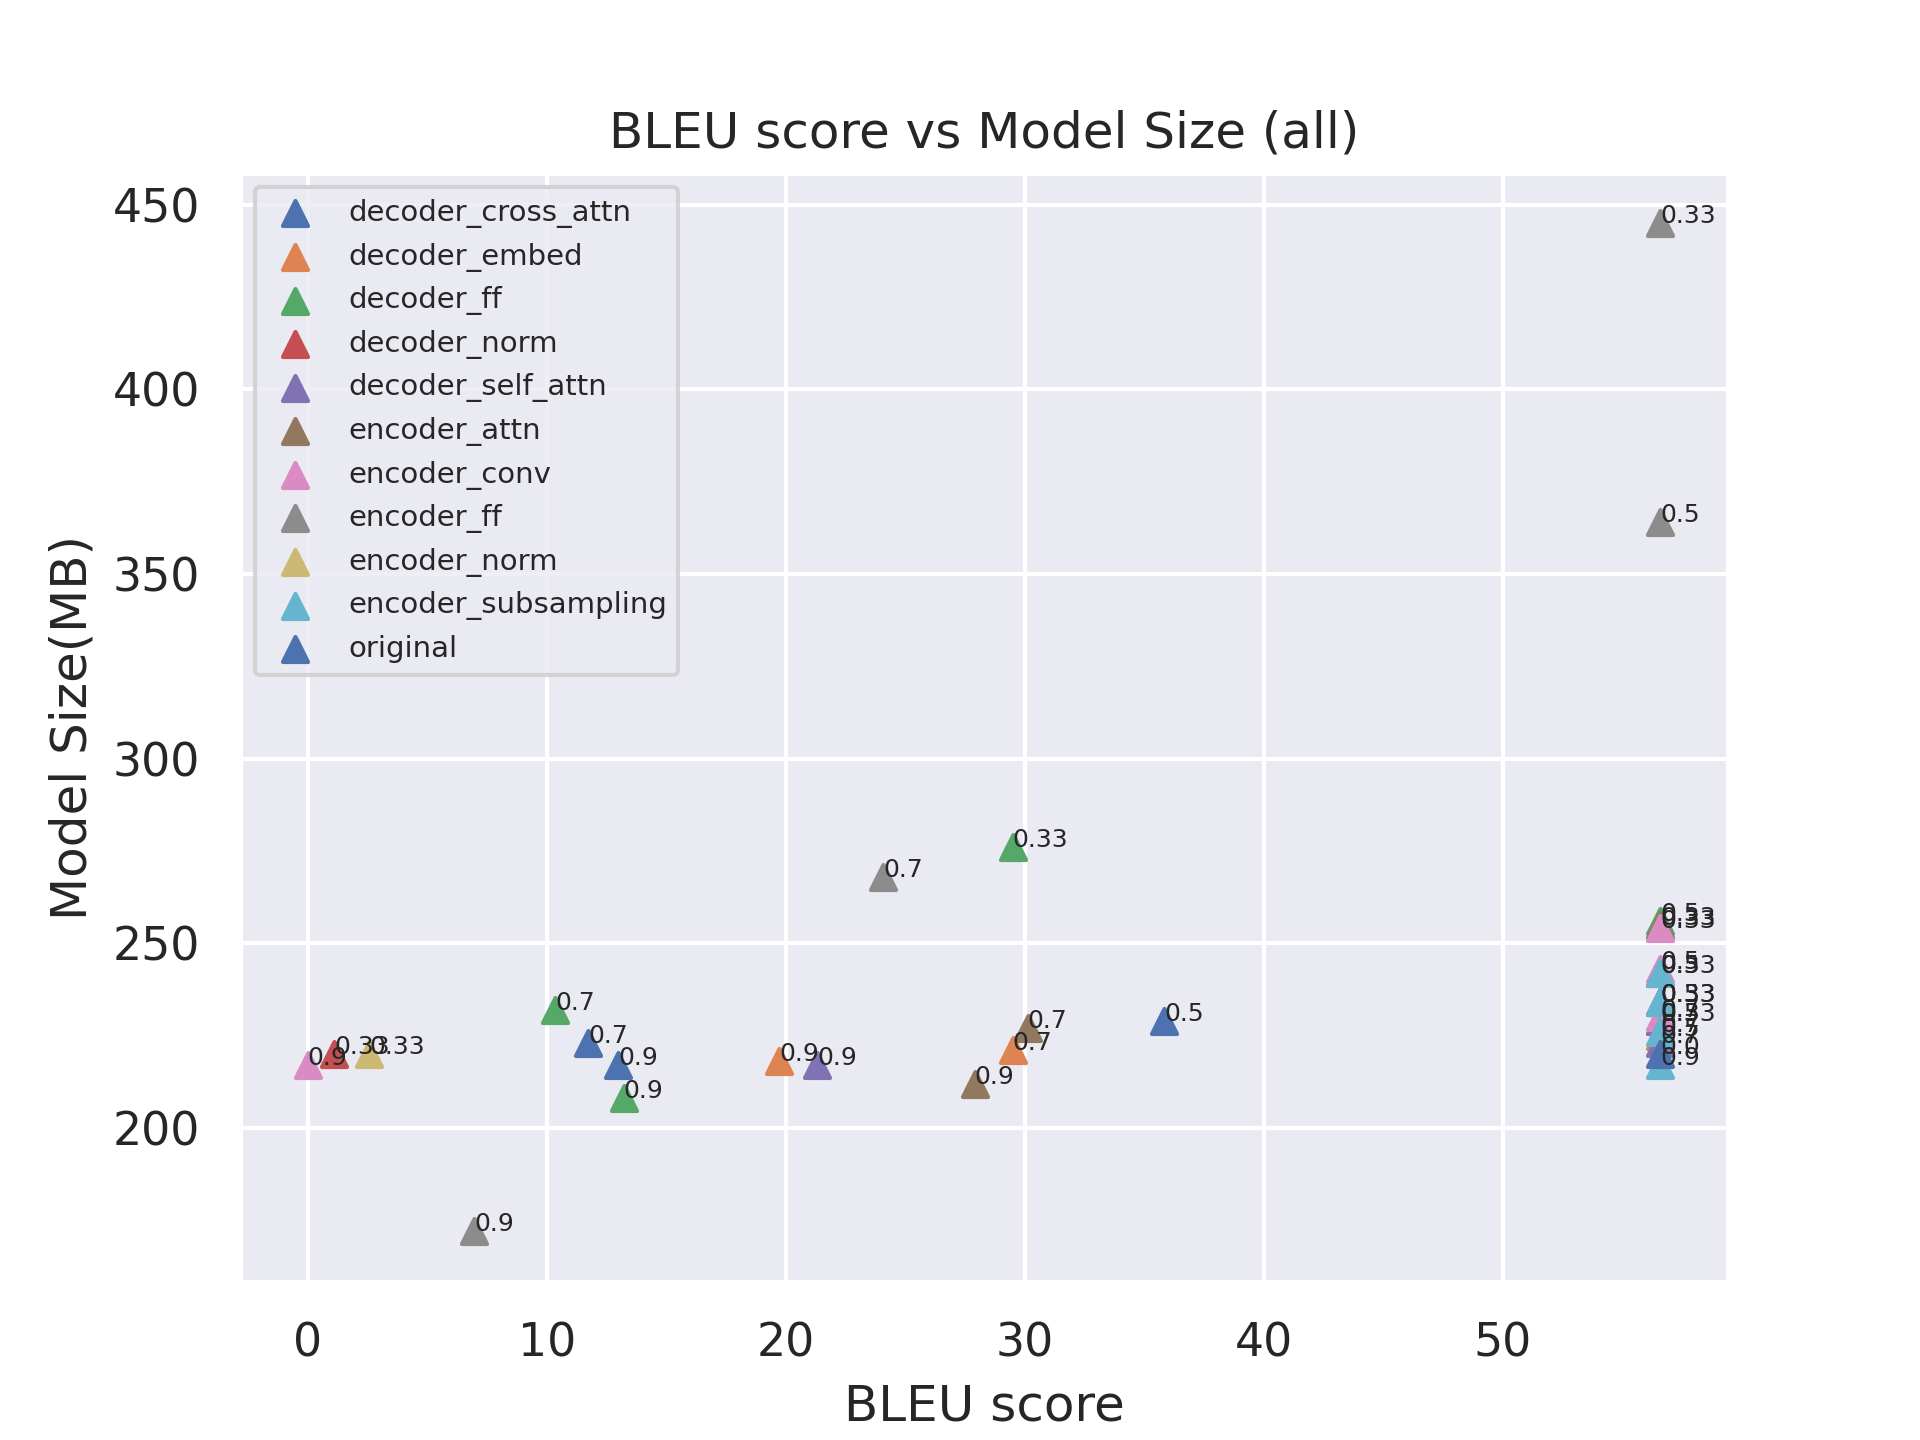
\includegraphics[width=\textwidth]{images/prun_modules/BLEU_vs_Model_Size_all.png}
        % \caption{BLEU vs. Disk Space (MB)}
    \end{subfigure}
    \caption{Comparative Plots For Different Sparsity on Different Modules}
    \label{fig:prun_module_all}
\end{figure*}

From the plot (Figure. \ref{fig:prun_module_all}), we may be able to get to the conclusion that:
\begin{enumerate}
    \item When decoder’s module gets pruned, the model will likely have a large performance degradation. One explanation for this is that the decoder is larger than the encoder, and here the decoder acted like a machine translation module + ASR Decoder, thus the decoder is supposed to have a larger model space compared to encoder, which means that the decoder theoretically needs a lot of parameters. Even if we only prune 33\% of the decoder’s parameters, it is likely to cause underfitting.
    \item It seems that pruning about 33\% or even a little bit more parameters of the encoder will not cause a huge performance loss compared to the original model. We think that it might be due to the fact that here the encoder plays a lower-level acoustic feature extraction role, which theoretically does not need so many parameters. Thus pruning 30\% of them will not greatly affect the performance.
    \item An interesting thing here is that even if we pruned about 70\% of the self-attention module of the encoder, the model could still achieve a BLEU score which is higher than 20. We think the reason is similar to the point we mentioned just above, the encoder here is not responsible for most of the semantic feature extraction, thus its attention module does not need a large model space.
\end{enumerate}
Based on the experiment results and our analysis we designed an optimal solution that balances the sparsity and model’s performance, which is listed in Table~\ref{tab:pruning_config}.
This solution can achieve a BLEU score of about 42.

\begin{table}[h!]
\centering
\begin{tabular}{cc}
Component & Sparsity \\ \hline
Encoder\_subsampling    & 0.9    \\
Encoder\_conv & 0.7 \\
Encoder\_ff & 0.5 \\
Encoder\_attn & 0.5 \\
Encoder\_embed & 0.5 \\
Encoder\_self\_attn & 0.5 \\
Encoder\_cross\_attn & 0.33 \\
\end{tabular}
\caption{The optimal pruning strategy based on our experiment results}
\label{tab:pruning_config}
\end{table}




\subsubsection{ONNX runtime}


\begin{figure}[h!]
    \centering
    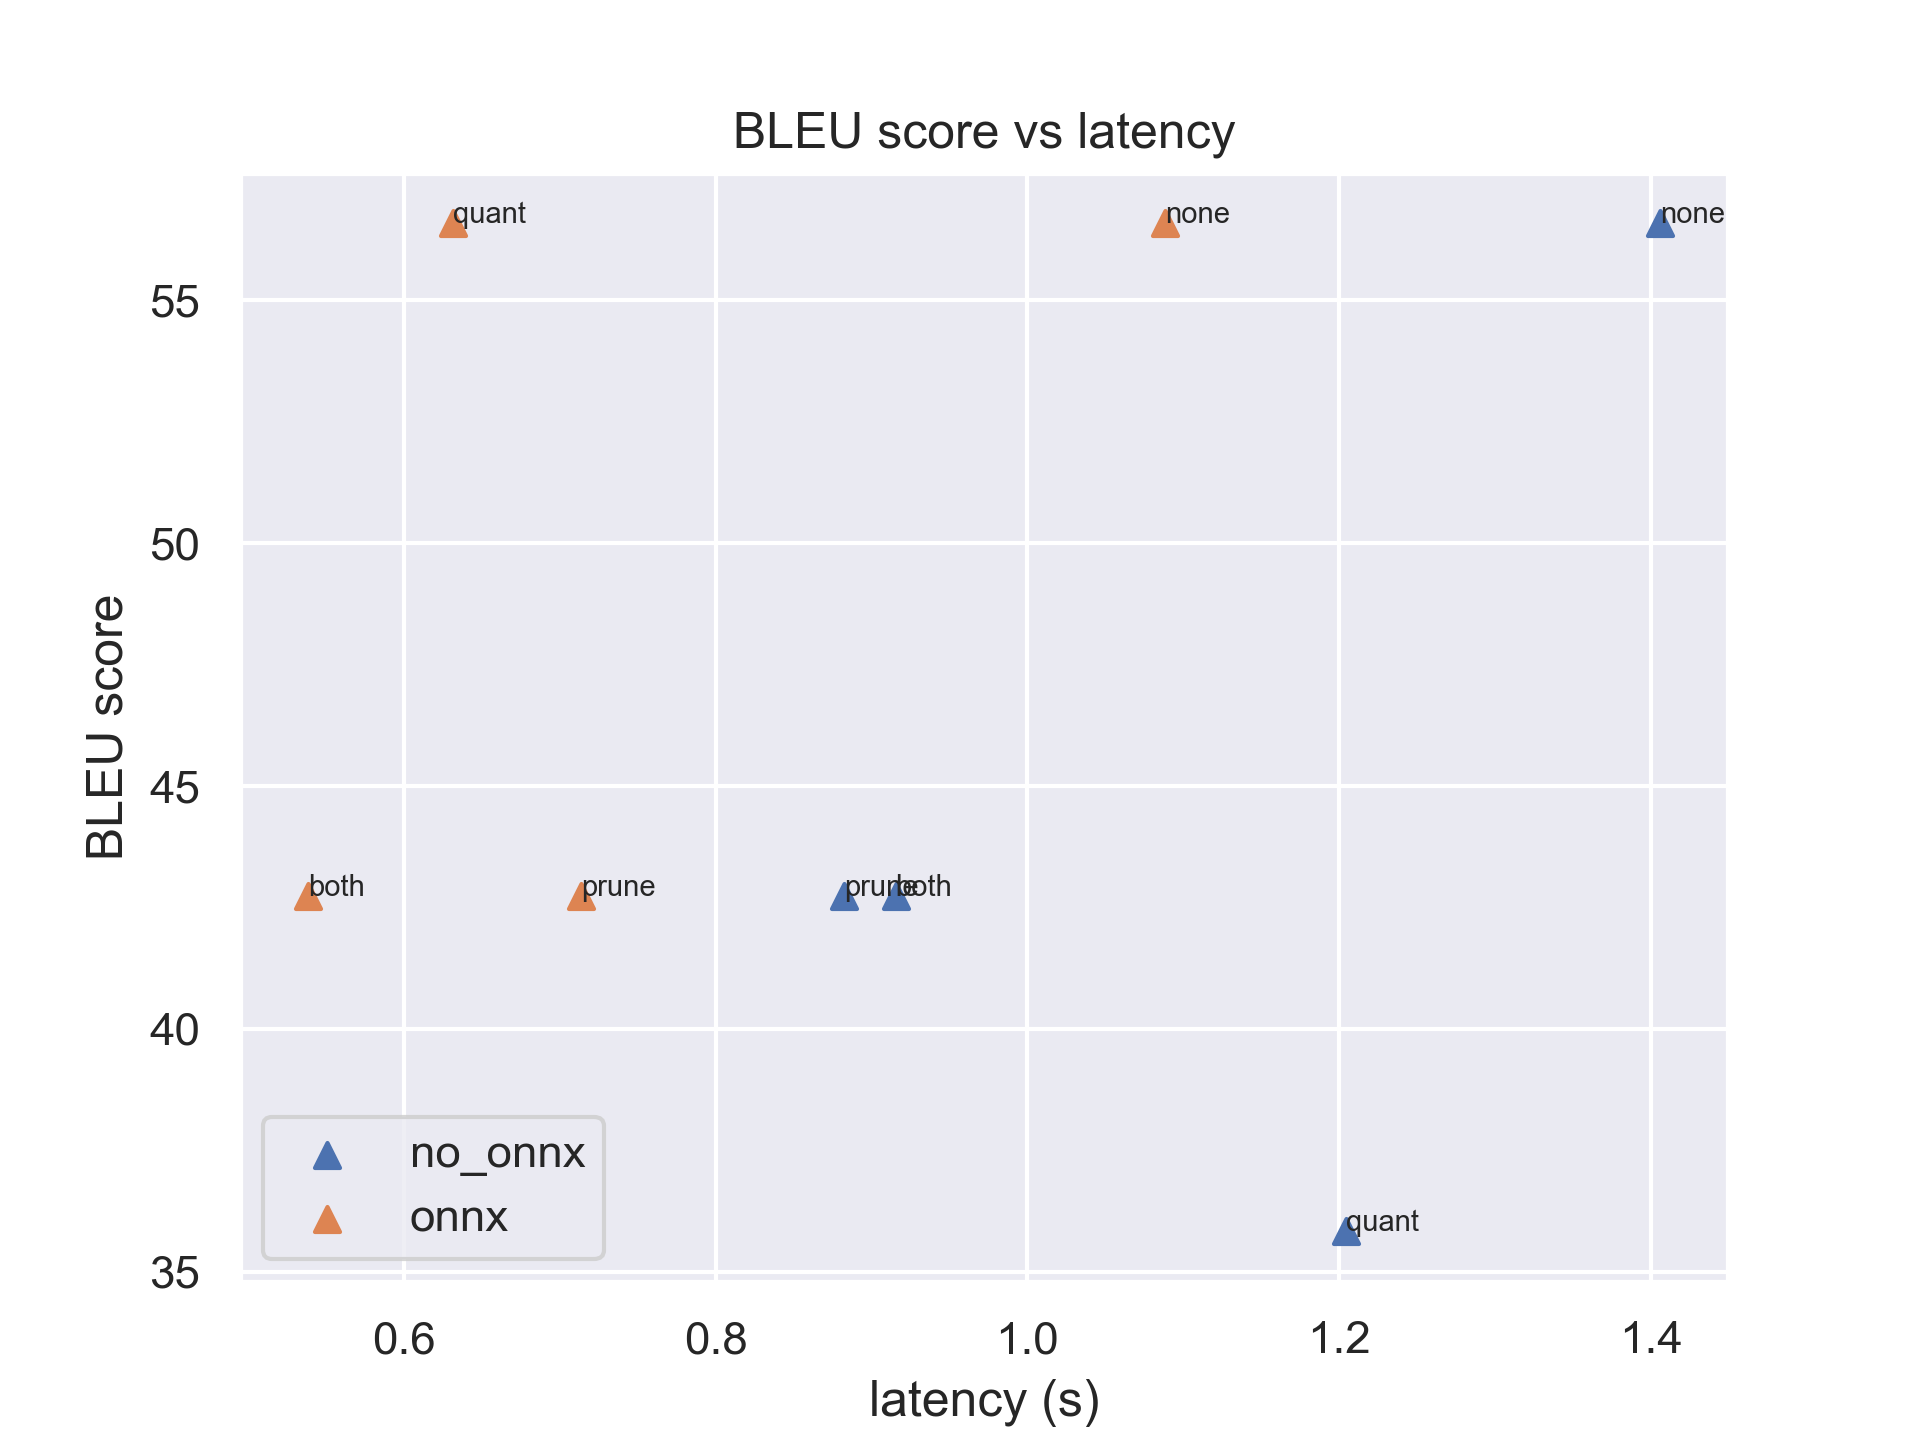
\includegraphics[width=0.5\textwidth]{images/ablation/BLEU_vs_latency.png}
    \caption{Ablation Study of quantization, pruning, and ONNX techniques}
    \label{fig:ablation}
\end{figure}

Figure~\ref{fig:ablation} shows the latency and BLEU scores of different combination of ONNX, quantization and pruning.
We can see that ONNX consistently reduces the inference time without any reduction of BLEU score, proving the effectiveness of this technique.
In addition, most of the performance degradation come from pruning, suggesting further refinement of the sparsity settings is required.
Interestingly, quantization using ONNX as a backend does not affect BLEU score, but this is not true if using PyTorch. We conjecture that ONNX's implementation of dynamic PTQ may be more stable than PyTorch's.



\subsection{Putting it together}


\begin{table}[h!]
\centering
\begin{tabular}{ccc}
Model Type             & BLEU & latency (s)  \\ \hline
Original               & 56.6  & 1.41        \\
PTQ + Pruning + ONNX   & 42.7  & 0.54        \\      
\end{tabular}
\caption{The most efficient model vs. the original model.}
\label{tab:final_product}
\end{table}

To get the most efficient model based on previous discussion, we apply component-wise pruning with settings shown in Table~\ref{tab:pruning_config}, convert it to ONNX format, and then apply 8-bit integer dynamic PTQ using ONNX runtime.
We benchmark this model and the results are shown in Table~\ref{tab:final_product}.
It's straightforward to see that these techqniues reduce the latency and model size by $-62\%$ and $-73\%$ respectively, and only led to a $-25\%$ relative reduction of the BLEU score.
We consider this reduction of BLEU score acceptable since a BLEU score of $42.7$ is very high among speech translation benchmarks.

% Our devices have limited processing power compared to cloud servers, which can impact the speed and accuracy of speech translation. Our adjustment is to optimize the machine learning models and algorithms for efficient on-device processing. Prioritize essential features and reduce resource-intensive processes. 
% In the future, we will extend the project by comparing end-to-end architecture and cascaded architecture. We will explore which architecture achieves better performance after applying model quantization and pruning. We will benchmark the performance of each model and try to understand and find the best trade-off between the accuracy and latency of each architecture.  

\subsection{Measuring Energy Use}

\begin{figure}[h!]
    \centering
    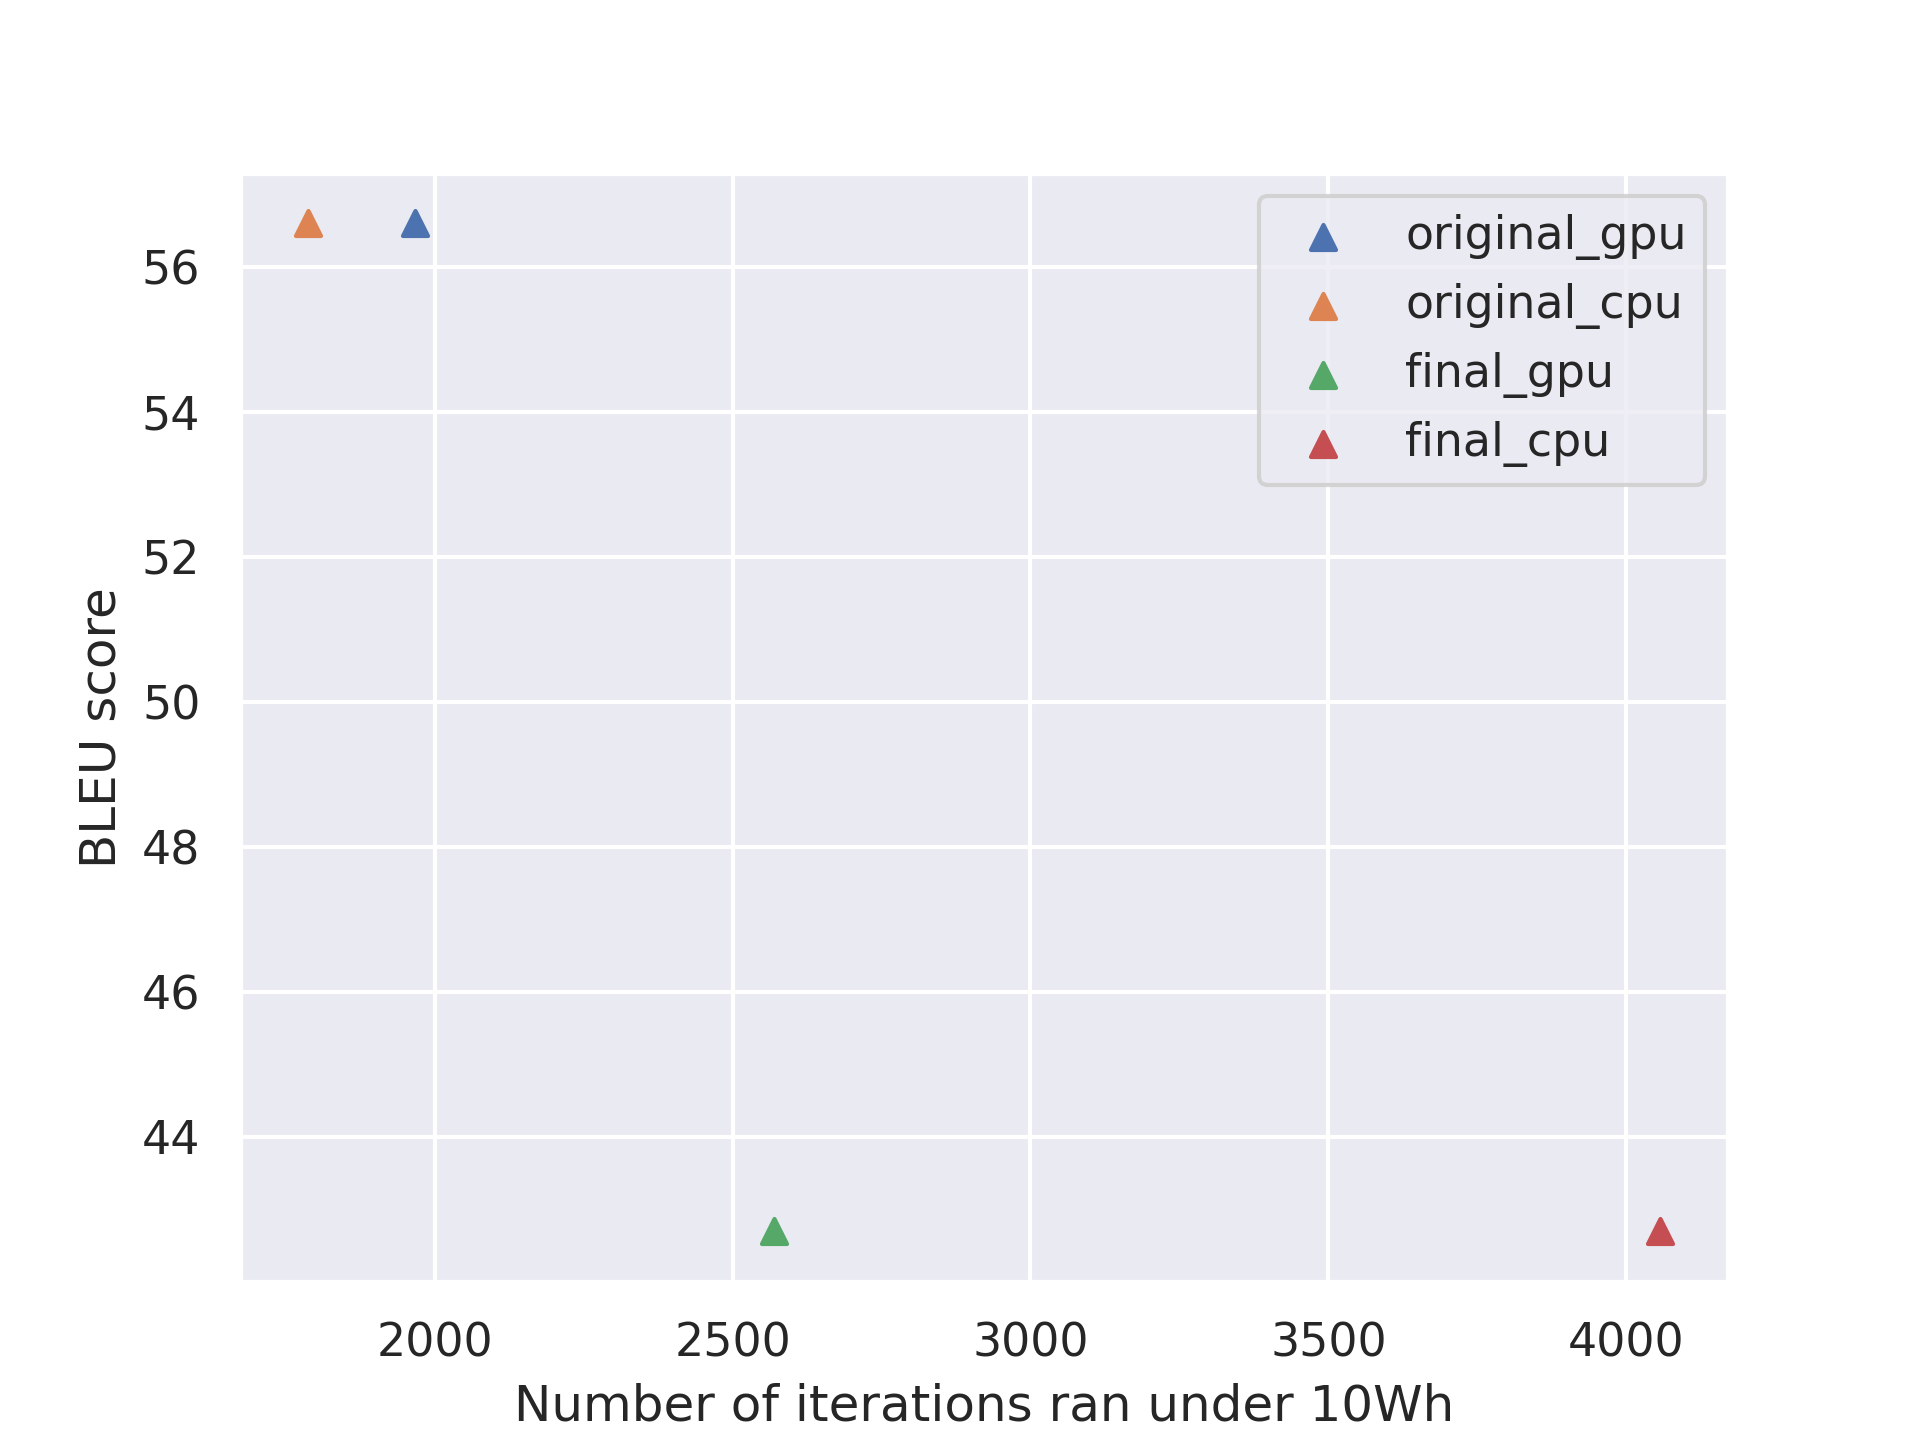
\includegraphics[width=0.5\textwidth]{images/under_10Wh.png}
    \caption{BLEU score vs. number of iterations under 10Wh}
    \label{fig:under_budget}
\end{figure}

% \textcolor{red}{TODO: analyze the graph}
The graph shows that for the original model, the GPU is slightly more energy-efficient than the CPU for inference. We think this might because that the GPU’s parallel computing mode is more efficient than the CPU’s sequential computing mode. Moreover, the 11th gen Intel CPU is not very energy-efficient. Therefore, for the original model, GPU is a better choice for inference.

After applying quantization, pruning, and ONNX optimization, our best model is much more energy-efficient than the original one with a small performance loss. Surprisingly, CPU outperforms GPU in terms of energy efficiency. This could be due to that the ONNX implementation is more optimized for the CPU’s Instruction Set Architecture (ISA), or maybe CPU handles low-resource tasks better. However, we do not have much context about the underlying architecture and implementation of these two platforms, so these are only speculations.


\subsection{Challenges}
In this project, we faced two main challenges. The first is that exporting the model to ONNX is cumbersome, mainly due to the beam search process. We used \textit{espnet\_onnx} as a starting point to make this easier, and the encoder and decoder are exported separately. The second challenge is that our experimentation with input size yielded surprising results. If time permits, we need to conduct more ablation studies to examine the reasons for the results for varying input size.


\subsection{Insights}
% \textcolor{red}{TODO: move to corresponding discussions}

In our project, we explored several optimization techniques for the on-device speech translation system based on ESPNet. Our insights revealed that 
\begin{itemize}
  \item Increasing the hop length of the input significantly reduces latency of conformer, while maintaining an acceptable level of performance with minimal information loss. Conversely, downsampling the original waveform led to great latency reduction but resulted in considerable performance degradation and substantial information loss (about 50\% compared to increasing hop length).
  \item Post-training quantization(PTQ) with 8-bit integers enhanced latency without damaging the BLEU score, whereas PTQ with 16-bit floats increases latency due to the underlying 32-bit float operations in x86 architecture.
  \item Pruning experiments indicated that while decoder layer are sensitive to pruning, which could lead to poor outputs. Certain layers like LayerNorm will cause a performance drop after pruning. Certain layers like LayerNorm and decoder self-attention could tolerate more aggressive pruning.
\end{itemize}




\subsection{Future Work}
In response to the potential decrease in BLEU scores resulting from pruning, our future work involves an in-depth exploration of hyperparameters to identify the most optimal settings. This may include Quantization-Aware training (QAT) and a meticulous search for hyperparameter configurations that mitigate the impact of pruning on model quality. 

Additionally, we will explore structured pruning, strategically assessing the removal of specific components to ensure that model efficiency is enhanced without compromising overall performance. 

What's more, our project will conduct a comprehensive investigation into the disparities between Torch and ONNX implementations of quantization. By comparing these frameworks, we aim to discern the subtle nuances in their approaches to quantization, providing valuable insights for further model refinement and optimization.


% \section{References}

\bibliography{custom}
\bibliographystyle{acl_natbib}


\end{document}
